\documentclass[runningheads]{llncs}

%%%%%%%%%%%%%%%%%%%% Non standard in llncs %%%%%%%%%%%%%

%\usepackage{appendix}
\usepackage{chngpage}
% Allows Diagram Sketching
%
\usepackage[all]{xy}
\usepackage{tikz}
%
% Comments
%
\usepackage{comment}

%
% Math symbols
%
\usepackage{amssymb}
\usepackage{amsmath}
\usepackage{amsthm}
%\newtheorem{theorem}{Theorem}
%
% Figures
%
\usepackage{wrapfig}
\usepackage{float}
\floatstyle{boxed}
\restylefloat{figure}
\usepackage{graphicx}
\usepackage{indentfirst}
%
% Algorithmic code
%
\usepackage{algorithmic}
\usepackage{algorithm}
\usepackage{listings}

\usepackage{hyperref}
\usepackage{cite}


\lstset{
captionpos=b, 
frame=bt,
basicstyle=\footnotesize,
tabsize=4,
morekeywords={split,join, drop,Bit,random}, 
keywordstyle=\color{blue},
breaklines=true}


%
% Colours to the revision process
%
\usepackage{color}
\definecolor{blue}{rgb}{0,0,1}
\definecolor{red}{rgb}{1,0,0}
\definecolor{black}{rgb}{0,0,0}



%Hyperlinks
%
\usepackage{hyperref}

%
% Local macros
%
\def\equiv{\Leftrightarrow}
\def\conv#1{#1^\circ}
\def\comp{\mathbin{\cdot}}
\def\just#1#2{\\ &#1& \rule{2em}{0pt} \{ \mbox{\rule[-.7em]{0pt}{1.8em} \small #2 \/} \} \nonumber\\ && }
\def\quotes#1{``#1''}
% -- to dos
\newcount\td \td=0 %  to-do counter
\long\def\Todo#1{\vskip 1ex\noindent\fbox{
\global\advance\td by 1
\textbf{To-do (\number\td):}\\~
\begin{minipage}{.75\textwidth}
#1
\end{minipage}
}\vskip 1ex}
% ----- shorthands ----
\def\eqref#1{(\ref{#1})}

%Revised
%
 
\long\def\revised#1{
\noindent\fcolorbox{green!20}{green!20}{
\begin{minipage}{\textwidth}
\textbf{\textcolor{red}{Revised}}\\~
#1
\end{minipage}

}}

% Demanded

\pagestyle{headings}



\graphicspath{{texinputs/imgs/}}

%%%%%%%%%%%%%%%%%%%%%%%%%%%%%%%%%%%%%%%%%%%%%%%%%%%%%%%%%%
%
% Title
%

\title{Chat Server}
\subtitle{PSD --- Paradigms... \\
        }

%
% Authors
%

\authorrunning{Ana Carvalho \and Vítor Duarte}
\author{Ana Paula Carvalho\inst{1}
       \and
        Vítor Enes Duarte\inst{2}
}
% Affiliation and Email 
\institute{Minho University, Portugal\\
           \email{pg25335@alunos.uminho.pt}
		   \and
		   Minho University, Portugal\\
		   \email{pg19643@alunos.uminho.pt}}



\begin{document}

\maketitle
%
% Abstract
%

\begin{abstract}
Awesome abstract 


\end{abstract}

%
%  Introduction
%

\section{Introduction}
This project aims at building a \textbf{chat service (server and client)}. The server are the multiple components of the system that interact among each other while being hidden from the user. The client complies all the ways to access the services available by the server. In this case, the client is usually a chat user that comunicates with the server via a protocol (text-based).

\subsubsection{Project Goals.}
This project aims at building a distributed chat service with the following features:

\begin{itemize}
\item \textbf{User registration}, given name and password; registration removal; a user should be authenticated to use the service;
\item \textbf{Choice of room} (from existing ones), to which text messages will be sent;
\item Sending of \textbf{private messages} to other connected users;
\item Have a simple \textbf{text-based protocol} to allow simple chat clients, being usable by telnet;
\item Have a \textbf{REST API} for management and description: e.g., room creation/removal, list of rooms, list of users in room;
\item Have a \textbf{notification API} to allow subscribing to relevant events: room creation/removal, user joining/leaving room;
\end{itemize}

\subsubsection{Report structure.}
Bearing this in mind, this report will fistly address the theory behind this work in section \ref{sec:paradigms}; It will then in \ref{sec:implementation} explain the system's architecture and implementation choices; In section \ref{sec:results} there will be some use cases and a description of some problems found; And, in section \ref{sec:conclusion} a final appreciation of the work will be made, together with some suggestions for improvement.

%
% Dropwizard
%

\section{Paradigms and Tools}
\label{sec:paradigms}




%
%  Implementation
%

\section{Implementation}
\label{sec:impl}

\begin{figure}
\centering
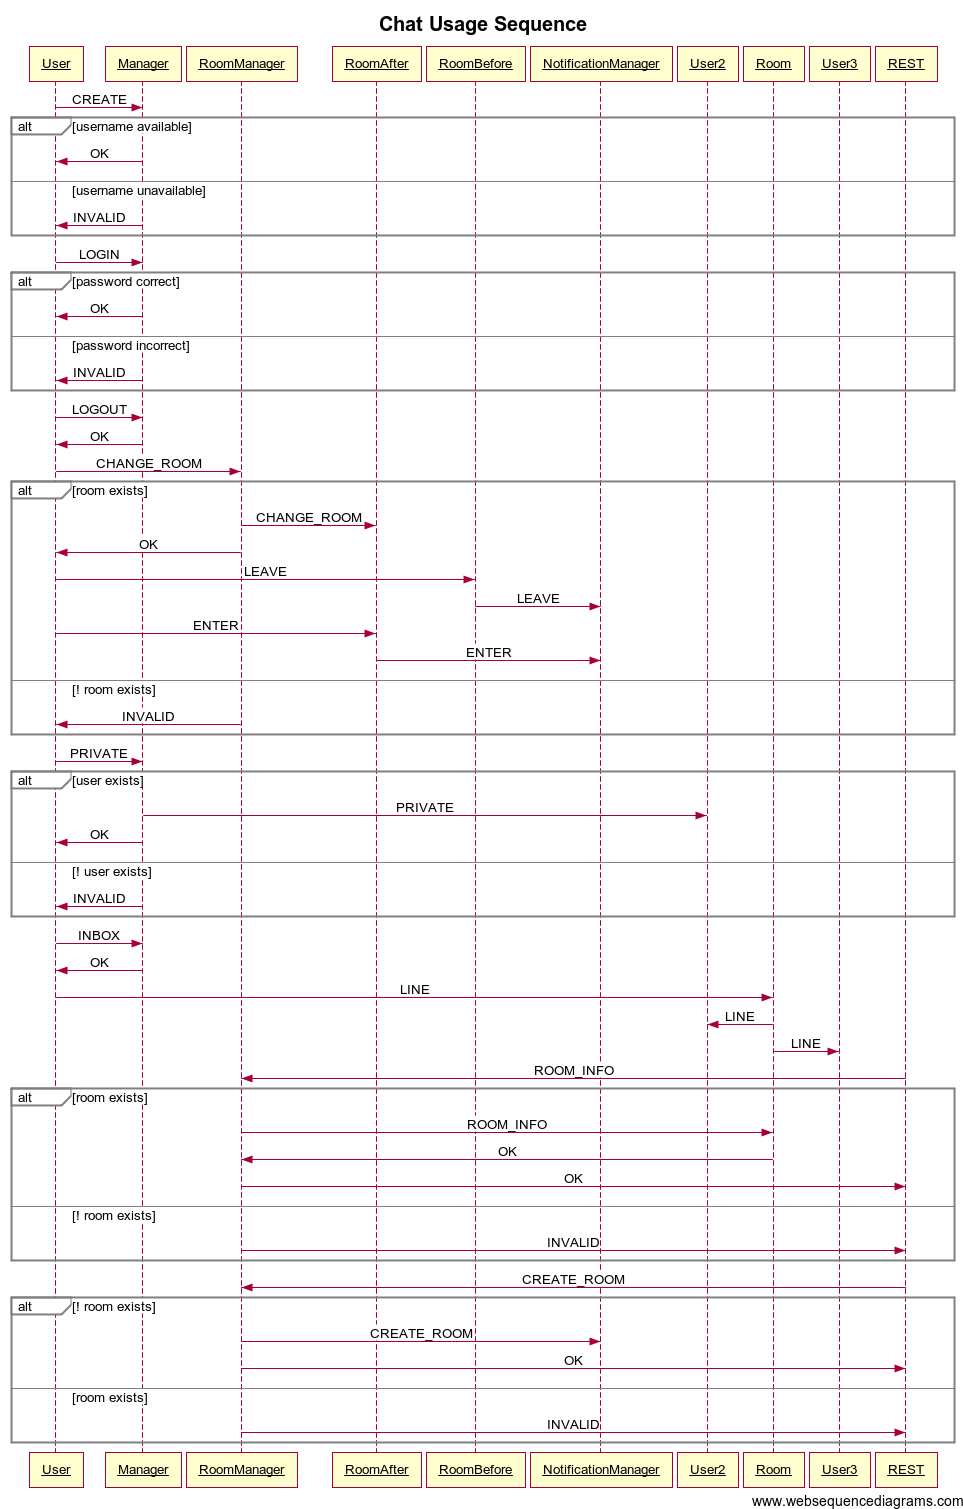
\includegraphics[width=1\textwidth]{seqdiag.png}
\caption{Sequence Diagram of Chat Usage}
\label{fig:seq_diag}
\end{figure}



%
% Telnet User
\subsection{User text protocol}

\begin{itemize}
\item cahsoicahscoiasc
\item :h/:help/:? - Lists all available commands\\
\item :cr/change new\_room - Change room\\
\item :logout - Logout \\
\item :login user pass - login to chat\\
\item :listrooms - Lists rooms\\
\item :listusers - Lists all users\\
\end{itemize}

%
% Rooms
\subsection{Chat rooms}




%
% Conclusions and Future Work
%



\section{Conclusions and Future Work}
\label{sec:concl}




%
% Bibliography
%

\bibliography{texinputs/bib}{}
\bibliographystyle{plain}


%\appendix

%\section{Curve over $\mathbb{F}_{23}$}
%\input{anexops.tex}
%\label{table}

%\section{Tests}
%\input{tests.tex}
%\label{tests}


\end{document}

